\subsection{Exemple 2 : Création et logique d'une tâches}
\label{subsec:exemple_2}

Afin de mieux comprendre le fonctionnement de l'ordonanceur et des tâches, un exemple
d'implémentation est donné ci-dessous. Cet exemple est composé de deux tâches :
\begin{itemize}
    \item \texttt{task1} : une tâche qui créer la tâche 2 et affiche un message
    d'état du programme.
    \item \texttt{task2} : une tâche simulant une opération prenant du temps.
\end{itemize}
On suppose que la fonction \texttt{HAL\_GetTick} retourne le temps écoulé en millisecondes
depuis le démarrage du programme.

\begin{lstlisting}[style=prog, frame=shadowbox, caption={Exemple asynchrone}, label={lst:ex_async},
    emph={[1]ASYNC_task1, ASYNC_task2, ASYNC_task1_init, ASYNC_task2_init, init_scheduler, add_task, kill_task, run_task,
    run_scheduler, HAL_GetTick, printf}, emphstyle={[1]\color{C}},
    emph={[2]SCHEDULER, TASK, TASK1_STATE, ASYNC_task1_CONTEXT, ASYNC_task2_CONTEXT}, emphstyle={[2]\color{E}}]
#include <stdbool.h>
#include "stm32f4xx_hal.h"
#include "scheduler.h"

typedef enum {
    TASK1_INIT,
    TASK1_WAIT,
    TASK1_END
} TASK1_STATE;

typedef struct {
    TASK1_STATE state;
    bool        task2_done;
    uint32_t    last_time;
} ASYNC_task1_CONTEXT;

typedef struct {
    bool         started;
    uint32_t     delay;
    uint32_t     last_time;
} ASYNC_task2_CONTEXT;


void ASYNC_task1_init(TASK *task);
void ASYNC_task2_init(TASK *task, uint32_t delay);
void ASYNC_task1(SCHEDULER *scheduler, TASK *task);
void ASYNC_task2(SCHEDULER *scheduler, TASK *task);


// =========================================


void ASYNC_task1_init(TASK *task) {
    ASYNC_task1_CONTEXT *context = (ASYNC_task1_CONTEXT*)task->context;

    context->state = TASK1_STATE_INIT;
    context->task2_done = false;
    context->last_time = 0;
}

void ASYNC_task2_init(TASK *task, uint32_t delay) {
    ASYNC_task2_CONTEXT *context = (ASYNC_task2_CONTEXT*)task->context;

    context->started = false;
    context->delay = delay;
    context->last_time = 0;
}


void ASYNC_task1(SCHEDULER *scheduler, TASK *task) {
    ASYNC_task1_CONTEXT *context = (ASYNC_task1_CONTEXT*)task->context; (*@\label{lst:ex_async:start-task1}@*)

    switch (context->state) {
        case TASK1_INIT:
            printf("Task 1 : Start\n");
            TASK *task = add_task(scheduler, ASYNC_task2);
            ASYNC_task2_init((ASYNC_task2_CONTEXT*)(task->context),
                        &context->task2_done, 5000);
            task->is_done = &(context->task2_done);     // Partage drapeau
            context->state = TASK1_WAIT;
            printf("Task 1 : Wait ");
            context->last_time = HAL_GetTick();         // Initialise timer
            break;
        case TASK1_WAIT:
            if (HAL_GetTick() - context->last_time > 200) {
                context->last_time = HAL_GetTick();     // Réinitialise timer
                printf(".");
            }
            if (context->task2_done) {                  // Vérifie tâche 2 terminée
                context->state = TASK1_END;
            }
            break;
        case TASK1_END:
            printf("\nTask 1 : End\n");
            kill_task(scheduler, task);
            break;
    }
}

void ASYNC_task2(SCHEDULER *scheduler, TASK *task) {
    ASYNC_task2_CONTEXT *context = (ASYNC_task2_CONTEXT*)task->context;

    if (!context->started) {
        context->started = true;
        context->last_time = HAL_GetTick();             // Initialise timer
    }
    if (HAL_GetTick() - context->last_time > context->delay) {
        kill_task(scheduler, task);                     // Drapeau *is\_done mis à jour
    }
}

// =========================================================

int main() {
    SCHEDULER scheduler;                                      (*@\label{lst:ex_async:start-init-scheduler}@*)
    init_scheduler(&scheduler);                               (*@\label{lst:ex_async:end-init-scheduler}@*)

    TASK *task = add_task(&scheduler, ASYNC_task1);           (*@\label{lst:ex_async:start-init-task1}@*)
    ASYNC_task1_init((ASYNC_task1_CONTEXT*)(task->context));  (*@\label{lst:ex_async:end-init-task1}@*)

    while (scheduler.length > 0) {
        run_scheduler(&scheduler); (*@\label{lst:ex_async:run}@*)
    }
    return 0;
}
\end{lstlisting}

\newpage

Cela produit le résultat suivant :
\begin{lstlisting}[style=terminal, frame=shadowbox, caption={Résultat xemple asynchrone}, label={lst:res_ex_async}]
Task 1 : Start
Task 1 : Wait .........................
Task 1 : End
\end{lstlisting}

\begin{minipage}{0.95\textwidth}
\begin{wrapfigure}{L}{0.35\textwidth}
\vspace{0.5cm}
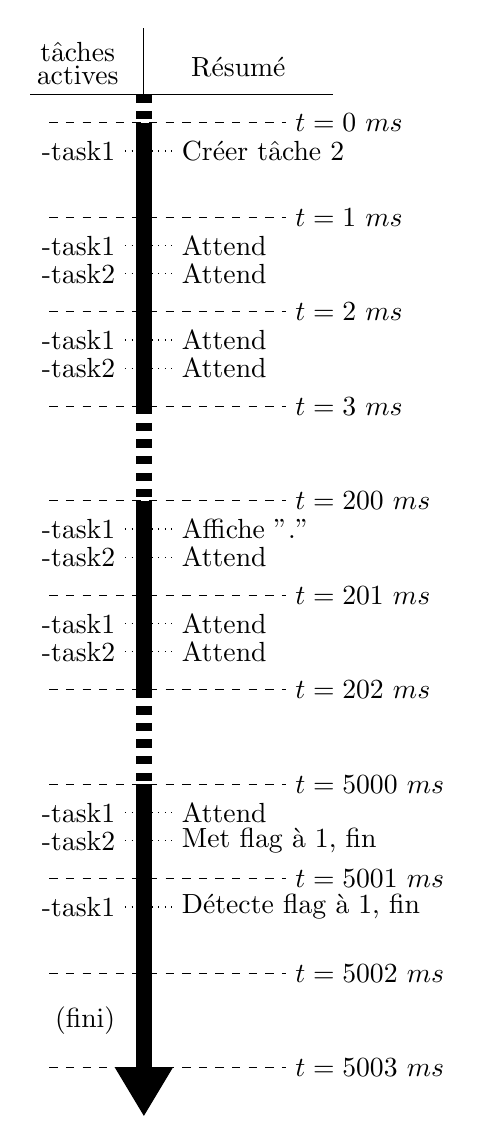
\begin{tikzpicture}[scale=1.2]

    % \draw [help lines] (-1, 0) grid (2, 12);

    \draw node at (-0.7, 11.75) {tâches};
    \draw node at (-0.7, 11.50) {actives};
    \draw node at ( 1, 11.595) {Résumé};

    % \draw [line width=0.5mm] (-1.2, 11.25) -- (2, 11.25);
    \draw (-1.2, 11.3) -- (2, 11.3);

    \draw  (0, 12) -- (0, 11.3);
    \draw [line width=2mm, dashed] (0, 11.3) -- (0, 11);
    \draw [line width=2mm        ] (0, 11) -- (0,  8);
    \draw [line width=2mm, dashed] (0,  8) -- (0,  7);
    \draw [line width=2mm        ] (0,  7) -- (0,  5);
    \draw [line width=2mm, dashed] (0,  5) -- (0,  4);
    \draw [line width=2mm        ] (0,  4) -- (0,  1);
    \draw [fill=black] (-0.3, 1) -- (0.3, 1) -- (0, 0.5) -- cycle;

    \draw [dashed] (-1, 11) -- (1.5, 11) node [right] {$t=   0 \ ms$};
    \draw [dashed] (-1, 10) -- (1.5, 10) node [right] {$t=   1 \ ms$};
    \draw [dashed] (-1,  9) -- (1.5,  9) node [right] {$t=   2 \ ms$};
    \draw [dashed] (-1,  8) -- (1.5,  8) node [right] {$t=   3 \ ms$};
    \draw [dashed] (-1,  7) -- (1.5,  7) node [right] {$t= 200 \ ms$};
    \draw [dashed] (-1,  6) -- (1.5,  6) node [right] {$t= 201 \ ms$};
    \draw [dashed] (-1,  5) -- (1.5,  5) node [right] {$t= 202 \ ms$};
    \draw [dashed] (-1,  4) -- (1.5,  4) node [right] {$t=5000 \ ms$};
    \draw [dashed] (-1,  3) -- (1.5,  3) node [right] {$t=5001 \ ms$};
    \draw [dashed] (-1,  2) -- (1.5,  2) node [right] {$t=5002 \ ms$};
    \draw [dashed] (-1,  1) -- (1.5,  1) node [right] {$t=5003 \ ms$};

    \draw [dotted] (-0.2, 10.7) node[left]{-task1} -- (0.3, 10.7) node[right]{Créer tâche 2};

    \draw [dotted] (-0.2,  9.7) node[left]{-task1} -- (0.3,  9.7) node[right]{Attend};
    \draw [dotted] (-0.2,  9.4) node[left]{-task2} -- (0.3,  9.4) node[right]{Attend};

    \draw [dotted] (-0.2,  8.7) node[left]{-task1} -- (0.3,  8.7) node[right]{Attend};
    \draw [dotted] (-0.2,  8.4) node[left]{-task2} -- (0.3,  8.4) node[right]{Attend};

    \draw [dotted] (-0.2,  6.7) node[left]{-task1} -- (0.3,  6.7) node[right]{Affiche "."};
    \draw [dotted] (-0.2,  6.4) node[left]{-task2} -- (0.3,  6.4) node[right]{Attend};

    \draw [dotted] (-0.2,  5.7) node[left]{-task1} -- (0.3,  5.7) node[right]{Attend};
    \draw [dotted] (-0.2,  5.4) node[left]{-task2} -- (0.3,  5.4) node[right]{Attend};

    \draw [dotted] (-0.2,  3.7) node[left]{-task1} -- (0.3,  3.7) node[right]{Attend};
    \draw [dotted] (-0.2,  3.4) node[left]{-task2} -- (0.3,  3.4) node[right]{Met flag à 1, fin};

    \draw [dotted] (-0.2,  2.7) node[left]{-task1} -- (0.3,  2.7) node[right]{Détecte flag à 1, fin};

    \draw          (-0.2,  1.5) node[left]{(fini)};


\end{tikzpicture}
\caption{Chronologie de l'exemple de programmation asynchrone}
\end{wrapfigure}

La figure ci-contre montre la chronologie de l'exemple. A noter que le temps
d'exécution est donné à titre indicatif et ne correspond pas à une échelle de temps réelle.

\vspace{0.5cm}

Le programme commence par créer et initialiser l'ordonanceur (ligne \ref{lst:ex_async:start-init-scheduler}
-\ref{lst:ex_async:end-init-scheduler}). C'est à dire que de la mémoire est alloué pour les tâches, que les
éléments du tableau \texttt{running} sont tous mis à \texttt{false} et que les autres variables de
l'ordonanceur sont également initialisées.
Ensuite, la tâche 1 est créée et ajoutée à l'ordonanceur. Cela est réalisé par l'appelle de la fonction
\texttt{add\_task}. Cette fonction cherche la première place libre dans la zone mémoire allouée à cet effet
dans le tas, initialise une nouvelle tâche à cet endroit et renvoie un pointeur vers cette dernière.
Le context de la tâche est ensuite initialisé par sa fonction relative (ici\newline \texttt{ASYNC\_task1\_init})
(lignes \ref{lst:ex_async:start-init-task1}-\ref{lst:ex_async:end-init-task1}).
Enfin, le programme entre dans une boucle et exécute la fonction \texttt{run\_scheduler} tant que
des tâches se trouvent active dans l'ordonanceur.

Au début de l'exécution, seule la tâche 1 se trouve active, elle est alors exécutée. Ligne
\ref{lst:ex_async:start-task1}, le contexte d'exécution de la tâche 1 est récupéré et l'état de la tâche
est vérifié. La plupart des tâches sont des machines à états finis \footnotemark. Dans le cas de la tâche
1, elle se trouve au début dans l'état \texttt{TASK1\_INIT}, elle affiche donc le message "Task 1 : Start",
créer la tâche 2 en l'ajoutant à l'ordonanceur, affiche "Task 1 : Wait" et passe à l'état \texttt{TASK1\_WAIT}.

La tâche 1 est alors mise en pause et la tâche 2 est exécutée. Cette dernière est une tâche simulant
une opération prenant du temps. Elle démarre tout d'abord un timer de 5000 ms et vérifie à chaque nouvelle
exécution si ce temps s'est écoulé. Lorsque c'est le cas, la tâche 2 se retire de l'ordonanceur. Quand la
tâche 1 détecte la fin d'exéctution de la tâche 2 (via la mise à jour du drapeau "\texttt{task2\_done}"), elle
affiche "Task 1 : End" et se retire également de l'ordonanceur. Dans le cas contraire, la tâche 1 continue
d'afficher des points toutes les 200 ms grâce à un timer propre. Ainsi, 25 points sont affichés correspondant
à un point toutes les 200 ms pendant 5 secondes. 

\end{minipage}

\footnotetext{Machine à état : Une machine à état (ou automate fini) est un modèle de calcul utilisé pour
représenter des systèmes avec un nombre fini d'états. Ce modèle est utilisé dans divers domaines comme les
protocoles de communication, les jeux vidéo, les systèmes embarqués, etc.}
